% CSE 291A Phase 1 report: Memory-Aware Agent Edge Serving.
% Build: pdflatex phase1_report.tex (twice), or upload report/ to Overleaf.
% Red \fillin{} markers are sections left for the author to complete.
\documentclass[10pt]{article}
\usepackage[margin=0.6in]{geometry}
\usepackage[small,compact]{titlesec}
\titlespacing*{\section}{0pt}{6pt}{3pt}
\usepackage[T1]{fontenc}
\usepackage{lmodern}
\usepackage{microtype}
\usepackage{graphicx}
\usepackage{booktabs}
\usepackage{tabularx}
\usepackage{enumitem}
\usepackage[font=small,labelfont=bf,skip=3pt]{caption}
\usepackage{subcaption}
\usepackage{xcolor}
\usepackage[hidelinks]{hyperref}
\setlist{nosep,leftmargin=1.2em}
\setlength{\parskip}{2pt}
\setlength{\textfloatsep}{6pt}
\setlength{\floatsep}{6pt}
\setlength{\abovecaptionskip}{2pt}
\graphicspath{{figures/}}
\newcommand{\fillin}[1]{\textcolor{red}{[TO FILL: #1]}}
\newcommand{\tok}{\,tok}

\title{\vspace{-1.6em}%
Project Option 1: Memory-Aware Agent Edge Serving\\
Phase 1 Report: Baseline and Measurement\vspace{-0.4em}}
\author{\quad Ethan Gross (200135377), CSE 291A Fall 2026}
\date{\vspace{-1.2em}}

\begin{document}
\maketitle

\section{Question, Setup, and Baseline}
\textbf{Question.} On a memory-limited personal machine, how do concurrency, growing contexts and idle time between
agent steps create memory pressure, and what limits completed agent work under a FIFO, fixed-concurrency baseline?

\textbf{Setup.} llama.cpp \texttt{llama-server}, pinned to release b11721 (commit \texttt{ff5a23376}), serving Qwen3-8B
(GGUF Q4\_K\_M) with an fp16 KV cache (144\,KiB per token), flash attention, and all layers solely on the GPU. I used my personal
Windows 11 desktop with an AMD Ryzen 9 7900X, an NVIDIA RTX 5070 Ti, and 32\,GB of DDR5 RAM. I disabled the GPU memory fallback to
system RAM so running out of VRAM fails instead of silently slowing down. Model, precision and server flags
were the same in every comparison.

\textbf{Memory budget.} All slots share one KV pool (\texttt{-kvu}) of 65,536 tokens ($\approx$9\,GiB, next to
$\approx$4.8\,GB of weights). The pool is allocated at startup, so GPU memory use is flat ($\approx$14,100\,MiB in every E2
run); what matters is how full the pool is. The server does not report this, so the runner tracks it from the tokens it
sends and receives.

\textbf{Baseline.} A Python asyncio runner with:
\begin{itemize}
\item FIFO admission and $K$ concurrent slots (server \texttt{-np}\,$=K$), so all queueing happens in the runner.
\item Pinned slots: a task keeps its slot, and its cached context, across tool calls.
\item Peak reservation: a task reserves its peak context when admitted; the queue head waits until it fits; a task
larger than the pool is rejected (\texttt{ctx\_overflow}).
\item A finished task's slot is erased before its reservation is freed.
\end{itemize}
Prompts are exact token arrays, with temperature 0 and fixed output lengths. Failures are classified (e.g.\
\texttt{timeout}, \texttt{kv\_exhausted}, \texttt{ctx\_overflow}) and never retried. Every request, task and 200\,ms
system sample is logged, along with the commit, server command and file hashes. Every run is checked: completed +
failed = planned tasks, and every prompt and output has its planned length.

\textbf{Workloads.} Defined in \texttt{configs/workloads/}; the same YAML and seed always produce the same tasks.
Prompts are exact token slices of Project Gutenberg books~\cite{gutenberg}. All mixes use 16 closed-loop agents and a
512-token shared prefix.

\noindent{\small
\begin{tabularx}{\linewidth}{@{}lccccX@{}}
\toprule
Mix & Steps & Initial context & Output/step & Tool output & Tool delay \\
\midrule
chat & 1 & 256--1,024 & 64/128/256 & -- & -- \\
long\_context & 1--2 & 6,144--12,288 & 128 & 256 & 1\,s \\
long\_output & 1 & 512--2,048 & 512/768/1,024 & -- & -- \\
agentic & 4--8 & 1,024--2,048 & 128/256 & 256--1,024 & lognormal, median 2\,s \\
blend & \multicolumn{5}{l}{40\% chat, 10\% long\_output, 20\% long\_context, 30\% agentic} \\
trace\_agentic & 5--12~\cite{continuum} & Mooncake trace~\cite{mooncake} & Mooncake (1--2,048) & lognormal, median 800~\cite{tracelab} & lognormal, median 0.23\,s~\cite{continuum} (heavy: 0.3\,s, $\sigma$ 2.98~\cite{tracelab}) \\
\bottomrule
\end{tabularx}}

\textbf{Workload Design.} The hand-designed mixes cover what the course asks for: short and long
contexts, short and long responses, and multi-step tasks with tool delays. The two trace mixes add realism. Public traces
have token counts and timings but no text, so they set the distributions while the tokens still come from the corpus:
\begin{itemize}
\item Context and output lengths: Mooncake's tool-and-agent production trace~\cite{mooncake}.
\item Step counts and trace\_agentic's tool delays: SWE-bench and BFCL agent runs reported by Continuum~\cite{continuum}.
\item trace\_agentic\_heavy's long-tailed tool delays and the tool output size: TraceLab's coding-agent
sessions~\cite{tracelab}.
\end{itemize}
The two trace mixes have identical tasks and differ only in tool delays. Details and limitations are in
Appendix~\ref{app:sources}.

\section{Experiments (171 runs, all valid)}
Each experiment answers one Phase 1 question from the course. E1 gives the cost model, E4 follows InferCept's question
of whether to keep or drop KV during tool calls~\cite{infercept}, and E7 was added after E2 to explain its slowdown. Each
experiment was piloted before the full grid.

{\small
\begin{tabularx}{\linewidth}{@{}lXl@{}}
\toprule
ID & What changes (everything else at baseline) & Reps \\
\midrule
E1 & Prompt 256--16,384 $\times$ output 32/128/512, $K=1$ (cost model) & 3 \\
E2 & $K \in \{1,2,4,8,16\}$ $\times$ six mixes; tasks per run $=\min(N, \max(20, 6K))$ & 3 \\
E3 & Context growth: 8 steps, initial context 1,024 vs 8,192, $K \in \{1,4\}$ & 2 \\
E4 & Tool delay 0/1/2/5/15\,s (agentic) and both trace mixes $\times$ slot mode pinned vs any, $K=4$ & 3 \\
E5 & Shared prefix 0 vs 4,096 $\times$ prompt cache on/off $\times$ erase vs keep finished slots, $K=4$ & 2 \\
E6 & Pool $c$ = 65,536/32,768/24,576/16,384 $\times$ admission gate on/off, trace\_agentic, $K=4$ & 2 \\
E7 & Microbenchmark: one active request vs idle KV in other slots (shared vs static split); batch size 1--16 & 3 \\
\bottomrule
\end{tabularx}}

\noindent Points are medians over reps, with min--max bars. One task failed unexpectedly (a client connection timeout in
E2, trace\_agentic, $K=8$); it is counted, and that setting is excluded when choosing the best $K$.

\section{Results}
\begin{figure}[t]
\centering
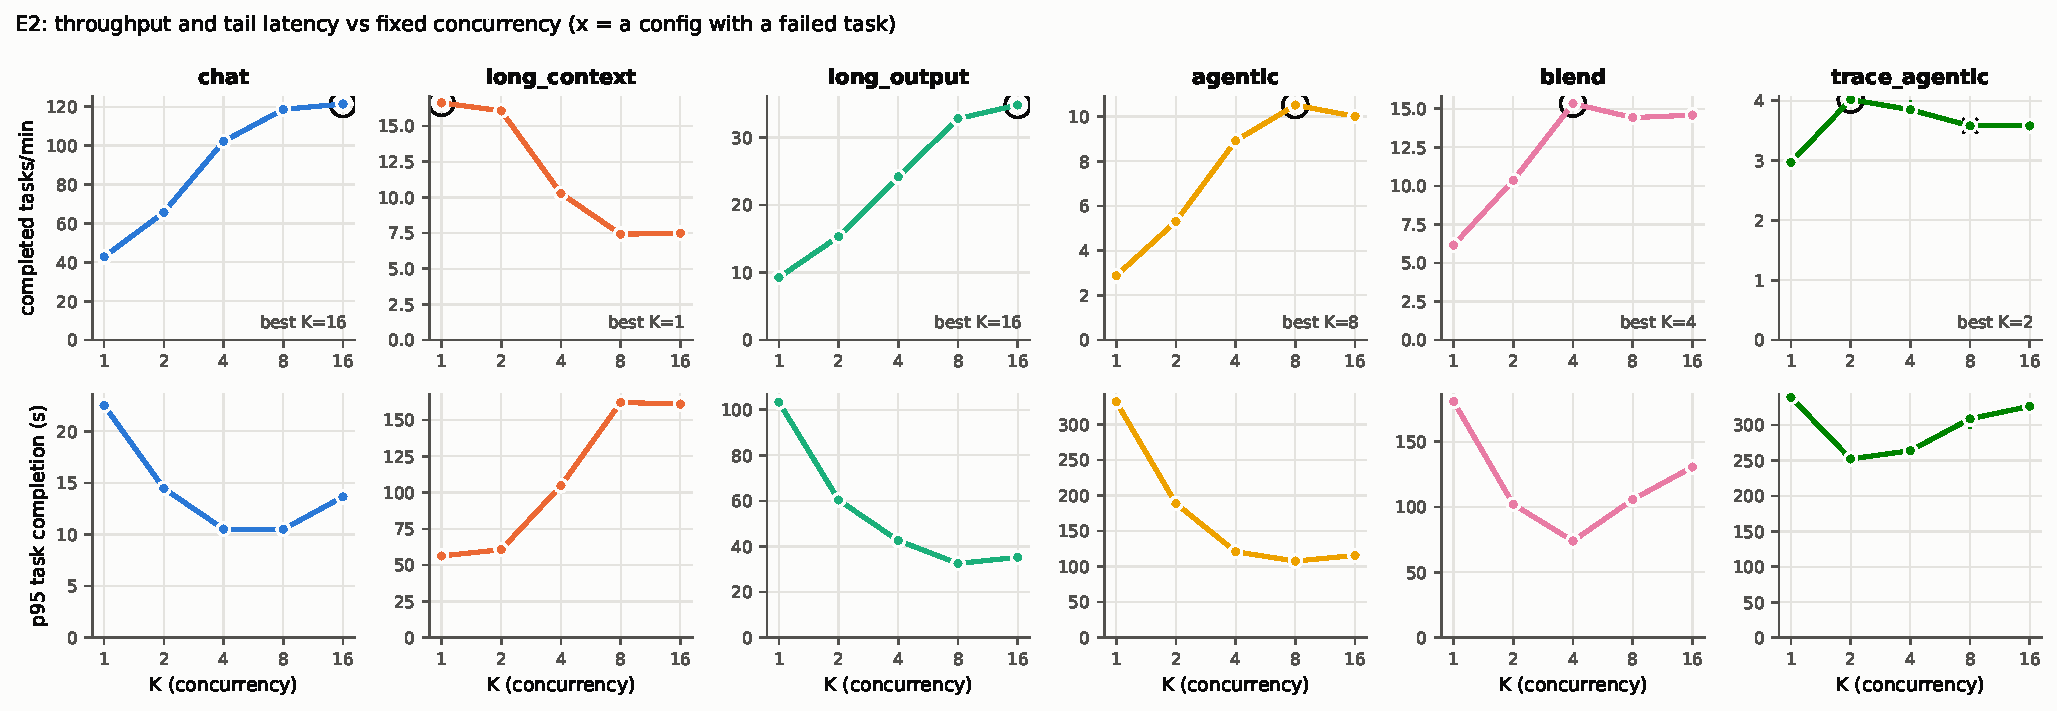
\includegraphics[width=\linewidth]{e2_throughput}
\caption{E2: completed tasks/min (top) and p95 task completion time (bottom) vs fixed concurrency $K$. Circle =
best fixed $K$ (highest throughput with no failed task; within 2\%, lower p95).}
\label{fig:e2}
\end{figure}

\textbf{Concurrency (Fig.~\ref{fig:e2}).} The best fixed $K$ depends on the mix: 16 for chat (42.8$\to$121.4 tasks/min)
and long\_output (9.3$\to$34.8), 8 for agentic (2.9$\to$10.5), 4 for blend (6.2$\to$15.3), 2 for trace\_agentic
(3.0$\to$4.0), and 1 for long\_context. long\_context gets \emph{slower} with concurrency (16.6$\to$7.4 tasks/min at $K=8$;
p95 56$\to$162\,s) because each request waits behind other slots' long prompts (decode 9$\to$220\,ms/token). At low $K$,
most of a task's time is spent waiting for admission. These best-$K$ values are the Phase 2 baseline.

\begin{figure}[t]
\centering
\begin{subfigure}{0.53\linewidth}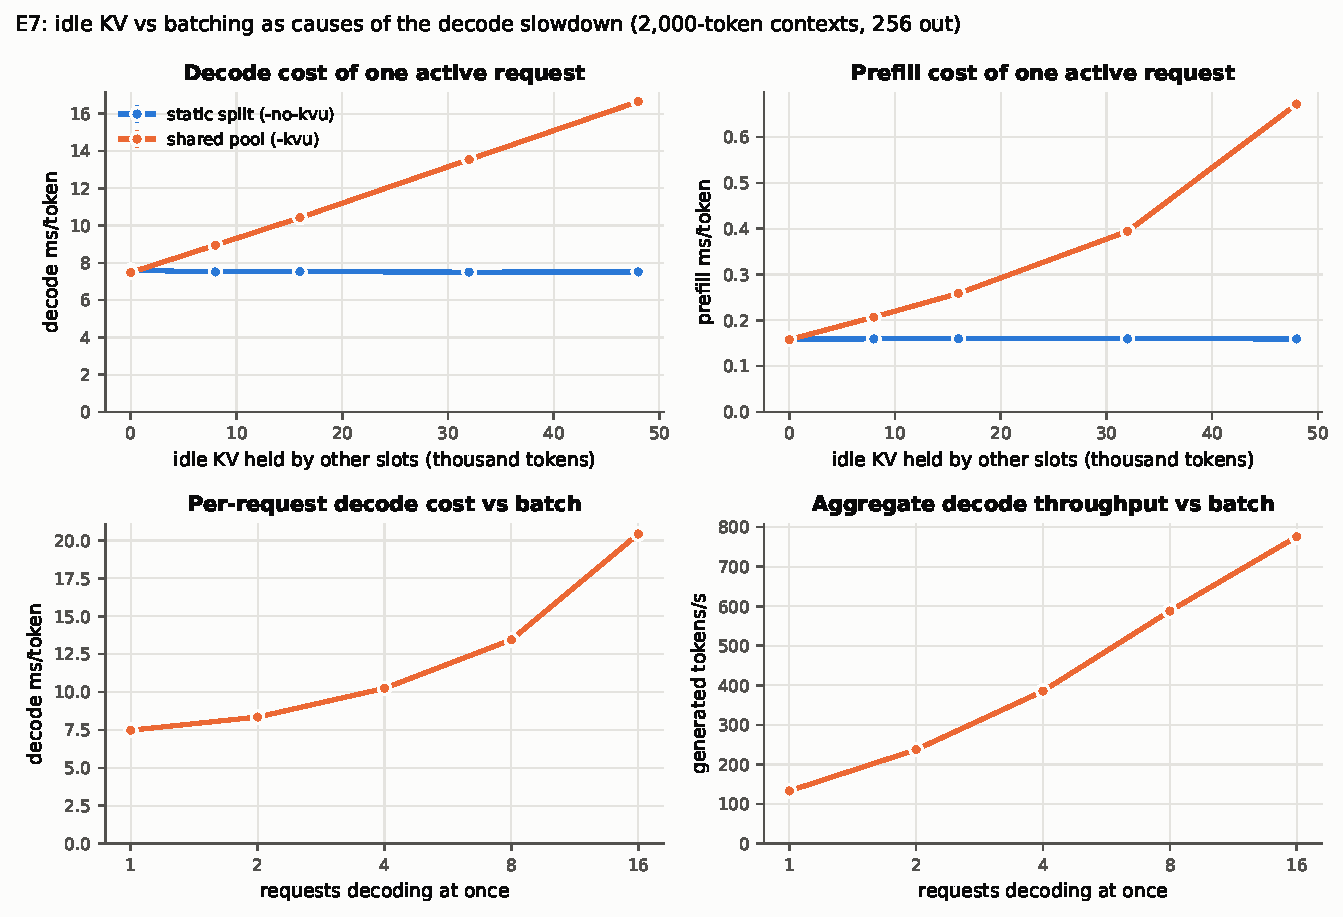
\includegraphics[width=\linewidth]{e7_idle_kv}\caption{E7: idle KV vs batching.}\end{subfigure}\hfill
\begin{subfigure}{0.45\linewidth}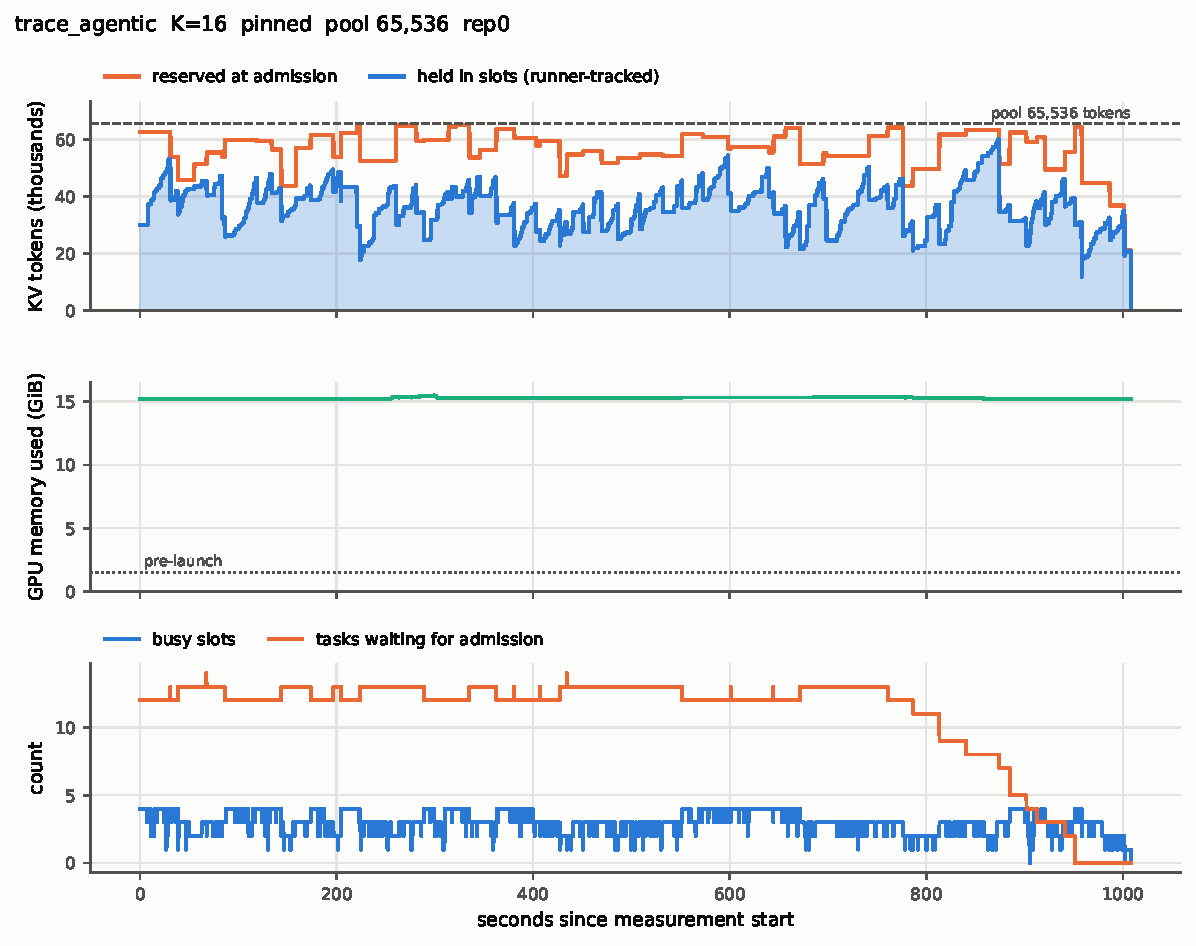
\includegraphics[width=\linewidth]{timeline_trace_agentic_K16_pinned_c65536_rep0}\caption{trace\_agentic, $K=16$, one run.}\end{subfigure}
\caption{The two causes of the bottleneck. (a) In the shared pool, idle KV in other slots slows the active request; with a
static split it does not. (b) Reserved KV (orange) stays near the pool limit while used KV (blue) is about 36k; at most 4
slots are busy while about 12 tasks wait.}
\label{fig:bottleneck}
\end{figure}

\textbf{Idle KV slows everyone (Fig.~\ref{fig:bottleneck}a).} With 48k idle tokens in other slots, the active request
decodes 2.2$\times$ slower (7.48$\to$16.66\,ms/token) and reads its prompt 4.3$\times$ slower (0.158$\to$0.672\,ms/token).
With a static split, neither changes. That is about +0.19\,ms per decoded token for every 1k idle tokens. Batching is
cheaper: 16 requests at once each decode at 20.4\,ms/token but produce 776 tokens/s in total, versus about 130 for one.

\textbf{Peak reservations block admission (Fig.~\ref{fig:bottleneck}b).} In trace\_agentic at $K=16$, about 56k tokens
are reserved on average but only 36k are used, so at most 4 slots are ever busy. agentic shows the same gap (59k vs
37.5k). This is why trace\_agentic stops improving after $K=2$.

\textbf{Context growth (E3).} Going from $K=1$ to 4 gives 2.3$\times$ throughput with 1k-token starting contexts but only
1.6$\times$ with 8k, as decode slows (9.6$\to$16.1\,ms/token) and used KV reaches 53k tokens.

\begin{figure}[t]
\centering
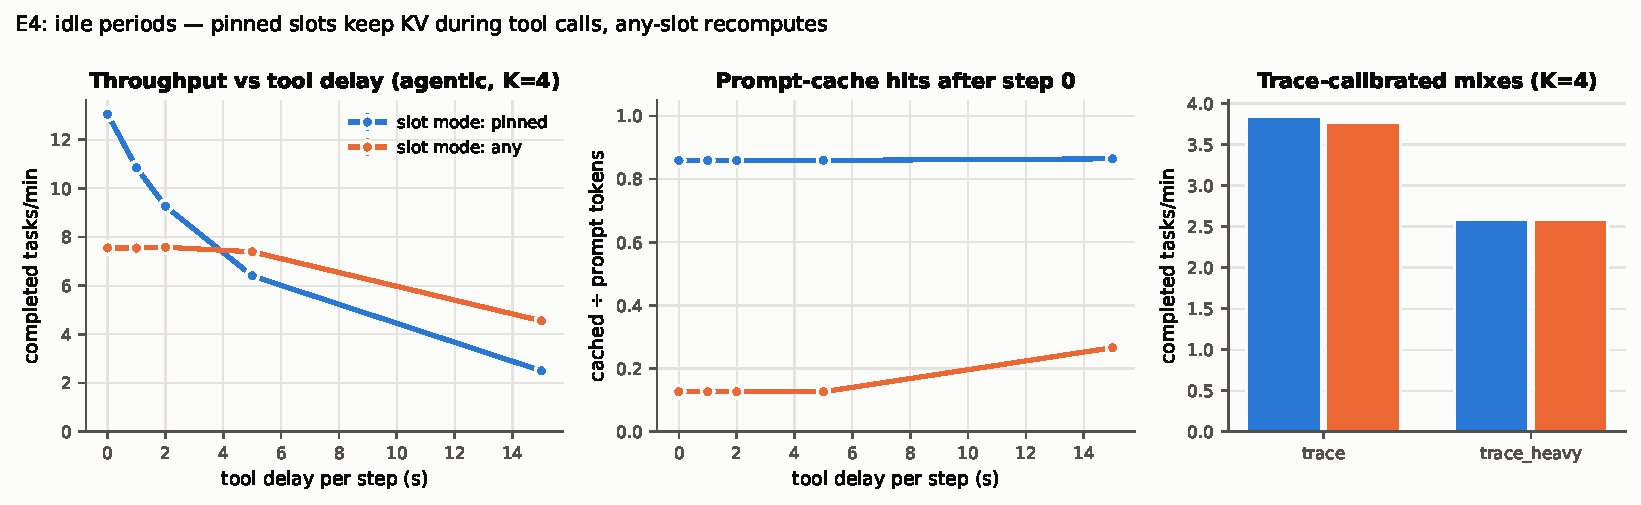
\includegraphics[width=0.8\linewidth]{e4_idle}
\caption{E4 ($K=4$): pinned slots keep a task's cache across tool calls; \emph{any} recomputes the prompt.}
\label{fig:e4}
\end{figure}

\textbf{Idle periods (Fig.~\ref{fig:e4}).} Pinned slots win when tool calls are short (13.0 vs 7.6 tasks/min at 0\,s)
because they recompute far less (114k vs 431k prompt tokens). Between 2 and 5\,s the order flips (5\,s: 6.4 vs 7.4;
15\,s: 2.5 vs 4.6), because pinned slots hold their KV for the whole tool call. On the trace mixes the two are within
3\%, so the slot choice matters little there.

\textbf{Reuse (E5).} The prompt cache matters most: turning it off cuts throughput by 26\%, or by 53\% with a
4,096-token shared prefix. Keeping finished slots helps only with a shared prefix (+14\%).

\textbf{Memory budget (E6).} Without the admission gate, 4 of 24 tasks fail at 65,536 tokens and all 24 fail at every
smaller pool, because one overflow fails every request in flight. With the gate, all 24 finish down to 32,768; at smaller
pools only tasks larger than the pool are rejected (1 and 8 tasks). Throughput at 16,384 covers only the 16 smaller
tasks, so it is not comparable.

\section{Dominant Bottleneck}
Completed work is limited by \emph{how the KV pool is held}, not by GPU compute power. There are two main causes I found while running the experiments:
\begin{enumerate}
\item Reserving each task's peak leaves about 36\% of reserved KV unused, so agentic mixes run well below $K$.
\item Agents waiting on tools keep their KV in the pool, which slows every active request
(Fig.~\ref{fig:bottleneck}a). Pinning helps for short tool calls and hurts for long ones (Fig.~\ref{fig:e4}).
\end{enumerate}
Raising $K$ isn't the solve-all solution. No single fixed $K$ is right for all mixes.

\section{Phase 2 Policy Directions}
Both policies fit the existing scheduler policy interface. Each is tested alone and together.
\begin{itemize}
\item \textbf{P1: Usage-based admission.} Reserve what a task holds now plus its next step, not its peak, and admit while
the free pool exceeds that need plus a headroom $H$. If no admitted task can continue, release the KV of the youngest
idle task (P2's mechanism). Motivated by the 56k-reserved vs 36k-used gap (Fig.~\ref{fig:bottleneck}b). The risk is
overflow, which fails every in-flight request (E6), so \texttt{kv\_exhausted} is a primary metric and $H$ is tuned on
dev seeds.
\item \textbf{P2: Idle-KV release.} When a tool call is expected to take longer than $\tau$, erase the task's slot
(\texttt{action=erase}) and recompute its prompt when it returns. Keeping costs about 0.19\,ms/token per 1k idle tokens
for every active request (E7); releasing costs one recompute at $\approx$5.5k tokens/s (E1). $\tau$ comes from this cost
model and should land near E4's 2--5\,s crossover. The expected delay uses only delays already observed, never the
pre-generated value.
\end{itemize}
\textbf{Evaluation.} Compare against FIFO at the best fixed $K$ per mix (chosen on dev seeds) and, for P2, against
always-pinned and always-any. On held-out seeds, report completed tasks, p50/p95 completion time, throughput, peak KV,
failures and policy overhead, with Poisson arrivals at several rates and changing mixes. Check that the largest tasks are
not unfairly delayed. Expected low-benefit cases: chat (no idle time) and the trace mixes for P2. The validity checks
ensure no gain comes from skipped tasks or shorter outputs.

\textbf{Reproducibility.} Sweeps: \texttt{python -m experiments.run\_sweep configs/experiments/E<n>\_*.yaml}
(resumable); E7: \texttt{python -m experiments.e7\_idle\_kv}; analysis: \texttt{python -m analysis.metrics E<n>} and
\texttt{python -m analysis.plots}. Runs used commit \texttt{66d6a71}; analysis code is at \texttt{36efa10}.

\clearpage
\appendix
\section{Timeline and milestones}
{\small
\begin{tabularx}{\linewidth}{@{}llXl@{}}
\toprule
\# & Date & Milestone & Status \\
\midrule
1 & 2026-10-29 & Stack pinned (llama.cpp b11721, Qwen3-8B Q4\_K\_M); runtime probes; VRAM vs pool size; shared-pool memory model agreed with TA & done \\
2 & 2026-11-01 & Deterministic workload generator, client, FIFO scheduler with policy interface, samplers, validity checks & done \\
3 & 2026-11-01 & Pool fixed at 65,536 tokens; pilots of all experiments valid; resumable sweep runner & done \\
4 & 2026-11-02 & Full E1--E6 (171 runs) and E7 & done \\
5 & 2026-11-03 & metrics and figures from raw logs & done \\
6 & 2026-11-04 & Phase 1 report submitted & done \\
\bottomrule
\end{tabularx}}

\section{Workload sources and calibration}\label{app:sources}
Pinned trace files, hashes and the fetch script are in \texttt{configs/trace\_manifest.json} and
\texttt{scripts/fetch\_traces.py}; the full rationale is in \texttt{docs/workload\_sources.md}.

{\small
\begin{tabularx}{\linewidth}{@{}p{0.2\linewidth}XX@{}}
\toprule
Source & What it provides & Used for \\
\midrule
Mooncake tool \& agent trace~\cite{mooncake} (Kimi, FAST'25; commit \texttt{3cca71d}, Apache-2.0) &
23,608 production requests with input and output token counts (input median 6,346, p90 16,805; output median 30, p90 507). &
Empirical draws of initial context (clipped to 256--16,384) and output per step (1--2,048) in both trace mixes. \\
Continuum~\cite{continuum} &
GPT-5 agent runs: SWE-bench 10.9$\pm$2.1 turns, tool time 925$\pm$3,550\,ms; BFCL web search 6.3$\pm$2.3 turns. &
Steps uniform 5--12; trace\_agentic tool delay lognormal (median 0.233\,s, $\sigma$ 1.66, clipped at 60\,s). \\
TraceLab~\cite{tracelab} &
4,265 Claude Code and Codex sessions: tool call median 0.3\,s, p90 13.6\,s; median append $\approx$857 tokens per step. &
trace\_agentic\_heavy tool delay lognormal ($\sigma$ 2.98, clipped at 120\,s); tool output lognormal (median 800, 16--8,192). \\
InferCept~\cite{infercept} &
Keep / discard / swap KV during tool calls. & Framing of E4 and Phase 2 P2 (not a workload source). \\
Project Gutenberg~\cite{gutenberg} &
Six public-domain books (1,674,729 tokens with the pinned tokenizer). &
Token content of every prompt and tool output, as exact token slices. \\
\bottomrule
\end{tabularx}}

\noindent\textbf{Limitations.} The trace mixes combine marginal distributions from three different systems; step count,
context, output and delay are drawn independently. Every task shares the same 512-token prefix, while real prefix
sharing is partial. Tool delays are clipped at 60 and 120\,s, which trims the heavy tail that makes idle retention
expensive. Outputs have forced lengths, so content and quality are not modelled (intended, for reproducibility).
Mooncake's arrival timestamps were not used; candidate sources for Phase 2's changing arrival rates are the Azure LLM
inference trace and BurstGPT.

{\small
\begin{thebibliography}{9}\setlength{\itemsep}{0pt}
\bibitem{mooncake} R.~Qin et al. Mooncake: A KVCache-centric Disaggregated Architecture for LLM Serving. FAST 2025.
Trace: \url{https://github.com/kvcache-ai/Mooncake/blob/main/FAST25-release/README.md}.
\bibitem{continuum} H.~Li et al. Continuum: Efficient and Robust Multi-Turn LLM Agent Scheduling with KV Cache
Time-to-Live. arXiv:2511.02230. \url{https://arxiv.org/abs/2511.02230}.
\bibitem{tracelab} TraceLab: Characterizing Coding Agent Workloads for LLM Serving. arXiv:2606.30560.
\url{https://github.com/uw-syfi/TraceLab}.
\bibitem{infercept} R.~Abhyankar et al. InferCept: Efficient Intercept Support for Augmented Large Language Model
Inference. ICML 2024.
\bibitem{gutenberg} Project Gutenberg. \url{https://www.gutenberg.org} (book ids 1342, 2701, 98, 84, 1661, 2600).
\end{thebibliography}}

\end{document}
